\documentclass{article}
\usepackage{graphicx}
\usepackage[utf8]{inputenc}
\begin{document}

\title{Progetto Programmazione avanzata e paradigmi \\ Indicizzazione documenti}

\author{Luca Guerra}

\maketitle

\section{Introduzione}
Si vuole sviluppare un'applicazione in grado di indicizzare in una struttura dati, situata in memoria centrale, le parole contenute in diversi documenti di testo. Grazie a questa struttura dati sarà possibile determinare in maniera veloce quali documenti contengono le parole cercate.

\section{Visione del problema}
Ho seguito un design di progettazione bottom-up, cercando fin da subito di individuare le varie entità a cui assegnarre i diversi compiti.\\
In particolare ho individuato i seguenti blocchi di lavoro (Task):
\begin{itemize}
  \item individuazione dei file da indicizzare
  \item indicizzazione delle parole presenti nei file trovati
  \item ricerca di una parola nei vari file
\end{itemize} 
I primi due Task possono essere realizzati in parallelo, mentre il terzo dovrà attendere il termine dei primi due (per evitare di dare una risposta incompleta).

\section{Soluzione al problema}

Per rendere il sistema più performante, ho deciso di sfruttare una \textbf{BlockingDeque}, questa verrà utilizzata come contenitore dei vari documenti da indicizzare. Il flusso di lavoro sarà il seguente: \\
Allo start dell'indicizzazione avrò un processo che naviga tutto l'albero partendo dalla root, la root sarà data in ingresso dall'utente, per realizzare questo Task sarà sufficiente un unico thread, dato che la navigazione rispetto l'indicizzazione sarà molto più veloce. Questo processo aggiungerà file alla lista, i vari processi indicizzatori rimarranno in attesa di nuovi file, appena questi saranno presenti li prenderanno e inizieranno a indicizzare in una hashtable. In questa soluzione l'hashtable sarà la nostra memoria condivisa, prendendo come assunto che questa struttura dati non diventerà mai più grande della memoria centrale dell'elaboratore. Ovviamente l'accesso a questa memoria dovrà essere mantenuto mutualmente esclusivo(garantito dalla LinkedBlockingDeque).
Per indicizzare nella hashtable avremo: la parola come chiave, associata a questa avremo una lista di stringhe rappresentanti tutti nomi dei documenti che contengono la parola chiave.\\
Terminata questa prima parte, il sistema è pronto a rispondere alle varie query consultando la hashtable (anche questo verrà fatto da un solo thread).

\section{implementazione}
Il progetto è stato suddiviso in 5 classi principali:
\begin{itemize}
  \item Gui
  \item ManageIndexer
  \item FileLoader
  \item Indexer
  \item Blackboard
\end{itemize}

\subsection{Gui}
La classe Gui si occupa della gestione dell'interfaccia grafica, in particolare notiamo la gestione dei Listener per lo \textbf{start}, \textbf{pause} e \textbf{stop} dell'indicizzazione. Questi, per gestire il comportamento dinamico dell'interfaccia, sfrutteranno lo SwingWorker implementato dalla classe ManageIndexer.
\subsection{Blackboard}
La blackboard è il contenitore per tutte le variabili statiche utilizzate per la sincronizzazione e comunicazione fra i vari processi.
\subsection{ManageIndexer}
La classe ManageIndexer, si occuperà di creare l'environment necessario all'indicizzazione, in particolare creerà l'executor, tutti gli indicizzatori e il loader dei file. Terminata la fase di creazione metterà in esecuzione il FileLoader attraverso l'Executor, la prima operazione del FileLoader sarà quella di segnalare l'evento al ManageIndexer, il quale potrà mettere in esecuzione gli altri thread nel pool, quando il loader segnalerà il termine del caricamento avrà inizio il tracciamento in una progress bar dell'avanzamento dell'indicizzazione (prima non era possibile dato che non avevamo il numero totale degli elementi). Una volta che l'executor avrà concluso il suo lavoro e si sarà spento, il ManageIndexer potrà terminare e dare il via alle query.
\subsection{FileLoader}
Questa entità sarà il processo che si occuperà del caricamento in una LinkedBlockingDeque dei File da indicizzare, la prima operazione che esegue al run è la signal della sua partenza, in questo modo consentirà il run degli indicizzatori (sfruttando una FixedThreadPool il numero degli indicizzatori realmente attivi, mentre è attivo il loader, sarà sempre il numero dei thread massimo meno uno, appena il loader finisce lascia il posto all'ultimo processo). Il FileLoader aggiungerà i vari file alla lista, una volta terminato metterà in lista un File particolare che verrà identificato come di terminazione, seguendo il "pattern" di spegnimento poison pills. Una volta inserita la "poison pill", farà una signal per consentire al ManageIndexer di iniziare con il tracciamento dell\textsl{}o stato di avanzamento dell'indicizzazione.
\subsection{Indexer}
L'indexer rappresenta il processo indicizzatore del sistema, sarà questo che assieme ad altri suoi simili prenderà dalla queue il file, lo aprirà e inserirà le parole trovate in una hastable. Gli indexer vivono in un while(true), la sua interruzione seguirà il pattern pison pills appena un indexer trova la poison pill la reinserisce (per indicarlo anche ad eventuali altri) e rompe il while andando a fare una wait in una CyclicBarrier, una volta che tutti gli indexer avranno fatto una wait sulla barriera questa verrà rotta e i processi potranno terminare.

\section{Dinamicità grafica}
Il programma deve avere un'interfaccia dinamica che consenta, mentre è in corso l'indicizzazione, di mettere in pausa far ripartire e stoppare l'operazione. Per fare ciò non possiamo far svolgere i vari task al thread evt che si occupa dell'interfaccia ma dobbiamo sfruttare uno SwingWorker, questo realizzerà le operazioni in background con un'atro thread lasciando l'interfaccia grafica attiva e disponibile per gestire la pausa ecc..
In particolare, nel momento dello start partirà lo swingWorker impementato dal manageIndexer, questo a sua volta farà partire indicizzatori e loader.
Mentre l'indicizzazione elabora, è possibile premere pausa o stop. La pausa richiamerà il metodo pause dello swingworker che stopperà momentaneamente il thread, ovviamente non basterà perchè dovranno essere fermati anche tutti gli indicizzatori, questi leggeranno una variabile pause nella blackboard settata a true,  mettendosi in attesa in un CountDownLatch inizializzato a 1 che avrà come compito quello di farli ripartire tutti alla pressione dello start assieme al metodo resume dello SwingWorker.
Lo stop semplicemente richiama un metodo cancel dello SwingWorker il quale termina il thread il quale spegne l'executor e resetta la blackboard ai valori iniziali.

\section{Poison Pills}
Sfruttando la LinkedBlockingDeque è venuto naturale sfruttare il patter di spegnimento \textbf{poison pills}. Quando il FileLoader ha terminato l'inserimento, inserirà un file identificato di chiusura, questo sarà l'ultimo file preso dagli Indexer, il file farà capire all'indicizzatore che deve spegnersi, ovviamente prima di farlo dovrà reinserire la pill per indicare anche agli altri indicizzatori la fine del loro lavoro.

\section{Testing}

\subsection{performance}
Sfruttando il tool VisualVM ho constatato i tempi di esecuzione totale degli indexer:\\ \\
Macchina con i7 2GHz x64 QuadCore
\begin{tabular}{|c|c|}
\hline Numero parole & Tempo esecuzione(sec) \\ 
\hline 741593 & 1 \\ 
\hline 1405434 & 1 \\ 
\hline 2810868 & 2 \\ 
\hline 4216302 & 3 \\ 
\hline 
\end{tabular}  \\ \\
Macchina con i7 2GHz x64 QuadCore
\begin{tabular}{|c|c|}
\hline Numero parole & Tempo esecuzione(sec) \\ 
\hline 741593 & 4 \\ 
\hline 1405434 & 4 \\ 
\hline 2810868 & 5,3 \\ 
\hline 4216302 & 15 \\ 
\hline 
\end{tabular} \\

\begin{figure}[h]
\centering
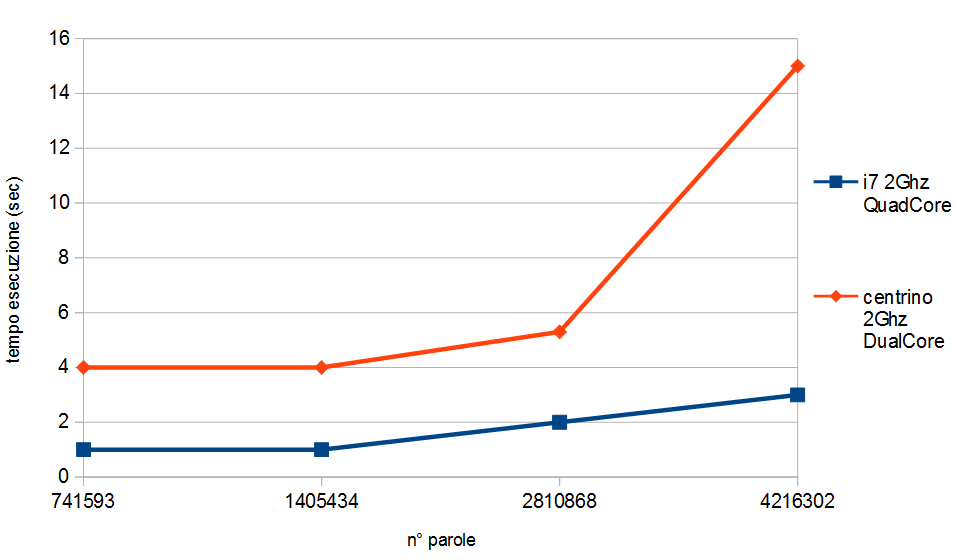
\includegraphics[width=0.9\linewidth]{./grafico_performance}
\caption[Performance workers]{Performance Indexers}
\label{fig:grafico_performance}
\end{figure}

Dai dati raccolti possiamo constatare un'incremento di performance dovuto al un numero maggiore di processori, nei primi range abbiamo uno scarto di 4 secondi, inoltre possiamo notare che per volumi bassi il tempo di esecuzione rimane costante, in pratica la parallelizzazione non porta benefici.\\
La cosa di particolare rilevanza per i nostri scopi è notare come, con 4 processori incrementando il numero di parole, nel range considerato il tempo di esecuzione rimane direttamente proporzionale al numero di parole, ovvero abbiamo un programma che scala bene con il numero di parole, mentre con un numero di processori minore il tempo di esecuzione tende ad aumentere in maniera esponenziale rispetto il numero di parole, quindi possiamo dedurre che il programma riesce a trarre vantaggio da un numero di processori più elevato.

\subsection{validazione}

Sono stati identificati vari Deadlock tramite lo strumento \textbf{Java Path Finder}.
Porto ad esempio lo startup dell'indicizzazione, per realizzare questa operazione ho sfruttato un pool fisso di thread pari al numero di processori disponibili sulla macchina + 1. In questo pool viene eseguito sia il FileLoader, sia i vari Indexer, questi, per sfruttare al meglio i processori, saranno in numero pari alla grandezza del pool. Sfruttando il Java Path Finder e in particolar modo il listener \textbf{DeadlockAnalyzer}, ho notato che seguendo un certo Path gli Indexer si bloccavano, lo scenario era il seguente:\\
Indicavo al Executor di eseguire prima il FileLoader poi i vari Indexer, lo start però non era gestito con una reale sincronizzazione, infatti nel path trovato da JPF, venivano fatti parire tutti gli index e poi il Loader, il File Loader però attendeva la terminazione dei processi per essere attivato dall'Executor, e dato il comportamento con poisol pill gli indexer non rilasciavano mai il pool mandando in DeadLock il sistema. Il problema è stato corretto sfruttando un semaforo evento, in pratica il ManageIndex comunica all'Executor di eseguire il processo FileLoader, attende l'ok dal semaforo (questo viene fatto scattare appena il FileLoader parte) e mette in esecuzione gli Runtime.getRuntime().availableProcessors() + 1 Indexer, ovviamente finché l'indexer non ha terminato il suo lavoro non saranno tutti attivi.
\\
Ho verificato anche proprietà di Safety, quale il numero di file trattati dai vari processi, tramite l'asserzione \textbf{assert progress == 4;} inserita nella blackboard.

NB:Per testare il modello del progetto ho sfruttato la seguente linea di comando:\\ 
\textit{java -jar percorsoCartellaJPF$\backslash$JPF$\backslash$jpf-core$\backslash$build$\backslash$RunJPF.jar\\ +site=percorsoConfigurazioneJPF$\backslash$JPF$\backslash$site.proprieties\\+shell.port=4242 C:percorsofilejpfdelprogetto$\backslash$DocumentIndexing.jpf } 
\end{document}